%%%%%%%%%%%%%%%%%%%%%%%%%%%%%%%%%%%%%%%%%
% qGAN Market Generator --- final presentation
% ZHAW CEC Quantum Computing, Spring 2026
%%%%%%%%%%%%%%%%%%%%%%%%%%%%%%%%%%%%%%%%%

\documentclass[
10pt,
xcolor=x11names,
aspectratio=169,
]{beamer}

%%%%%%%%%%%%%%%%%%%%%%%%%%%%%%%%%%%%%%%%%
% qGAN Market Generator --- preamble
%%%%%%%%%%%%%%%%%%%%%%%%%%%%%%%%%%%%%%%%%

%----------------------------------------
%   REFERENCES
%----------------------------------------
\usepackage[
    backend=biber,
    sorting=none,
    style=ieee
]{biblatex}
\usepackage{csquotes}
\addbibresource{sources.bib}

%----------------------------------------
%   FLOATS
%----------------------------------------
\usepackage{booktabs}
\usepackage{tabularx}
\usepackage{longtable}
\usepackage{graphicx}
\graphicspath{{figures/}}

%----------------------------------------
%   CAPTIONS
%----------------------------------------
\usepackage{caption}
\usepackage[subrefformat=parens]{subcaption}
\setbeamertemplate{caption}[numbered]
\captionsetup{justification=centering}

%----------------------------------------
%   ZHAW THEME
%----------------------------------------
\makeatletter
  \def\beamer@calltheme#1#2#3{%
    \def\beamer@themelist{#2}
    \@for\beamer@themename:=\beamer@themelist\do
    {\usepackage[{#1}]{\beamer@themelocation/#3\beamer@themename}}}

  \def\usefolder#1{
    \def\beamer@themelocation{#1}
  }
  \def\beamer@themelocation{}

\usefolder{zhawbeamer}
\usetheme{zhaw}
\usepackage{hyperref}


%----------------------------------------
%   DENSITY / SPACING ADJUSTMENTS
%----------------------------------------
% \usepackage{enumitem}
% \setlist[itemize]{leftmargin=*, topsep=2pt, itemsep=1pt, parsep=0pt}
% \setlist[enumerate]{leftmargin=*, topsep=2pt, itemsep=1pt, parsep=0pt}
% \setlist[itemize]{topsep=2pt, itemsep=1pt, parsep=0pt}
% \setlist[enumerate]{topsep=2pt, itemsep=1pt, parsep=0pt}
% Use beamer's native list spacing instead of enumitem
\setbeamertemplate{itemize items}[circle]
\setlength{\leftmargini}{1.5em}
\setlength{\leftmarginii}{1.2em}

% Smaller body fonts inside lists
\setbeamerfont{itemize/enumerate body}{size=\footnotesize}
\setbeamerfont{itemize/enumerate subbody}{size=\scriptsize}

% Tighten block spacing
\addtobeamertemplate{block begin}{}{\vspace*{-2pt}}
\addtobeamertemplate{block end}{}{\vspace*{-2pt}}

% Slightly smaller frame title
\setbeamerfont{frametitle}{size=\large}

% Reduce default skips
\setlength{\medskipamount}{4pt plus 1pt minus 1pt}
\setlength{\bigskipamount}{8pt plus 2pt minus 2pt}


% extra packages for math and tikz diagrams
\usepackage{amsmath, amssymb}
\usepackage{tikz}
\usetikzlibrary{positioning, arrows.meta, shapes.geometric, fit, backgrounds}
\usepackage{xcolor}

\definecolor{zhawaccent}{RGB}{0,100,170}

% small helper macros
\newcommand{\smi}{\mbox{SMI}}
\newcommand{\dax}{\mbox{DAX}}
\newcommand{\sap}{\mbox{S\&P\,500}}
\newcommand{\nikkei}{\mbox{Nikkei\,225}}
\newcommand{\qgan}{\mbox{qGAN}}

%----------------------------------------
%   PRESENTATION INFORMATION
%----------------------------------------
\title{Entangled Markets}
\subtitle{Hybrid Quantum GANs for Synthetic Multivariate Market Scenarios}
\author{Marcus Wunsch, Senior Lecturer at ZHAW School of Management and Law}
\date{13 May 2026}

\lfooter{ZHAW WBK Quantum Computing}
\mfooter{Final project presentation}

%----------------------------------------
\begin{document}

\frame[plain]{\titlepage}

\begin{frame}{Outline}
\tableofcontents
\end{frame}

%----------------------------------------
%   THEORETICAL CONTENT
%----------------------------------------
% !TEX root = ../main.tex

\section{Motivation}
\label{sec:motivation}
\frame[plain]{\sectionpage}

%----------------------------------------
\begin{frame}{Synthetic financial time series: a hard problem}
    \begin{columns}[T]
    \begin{column}{.55\textwidth}
        \textbf{Why generate synthetic returns?}
        \begin{itemize}
            \item Stress-testing portfolio strategies
            \item Backtesting under counterfactual regimes
            \item Risk modelling: VaR, Expected Shortfall
            \item ML training-data augmentation
        \end{itemize}
        \medskip

        \textbf{Why is it hard?}
        \begin{itemize}
            \item Returns are non-stationary, fat-tailed,
            volatility-clustered
            \item Cross-asset dependencies are non-Gaussian
            \item Historical data is scarce relative to the
            joint distribution's dimensionality
        \end{itemize}
    \end{column}
    \hfill
    \begin{column}{.40\textwidth}
        \begin{block}{Stylised facts}
            \begin{itemize}
                \item $\sim 0$ ACF in returns
                \item Strong positive ACF in $|r_t|$ and $r_t^2$
                (volatility clustering)
                \item Excess kurtosis: heavy tails
                \item Slight negative skew
                \item Asymmetric tail dependence
            \end{itemize}
        \end{block}
    \end{column}
    \end{columns}
\end{frame}

%----------------------------------------
\begin{frame}{The quantum hypothesis}
    \begin{columns}[T]
    \begin{column}{.55\textwidth}
        \textbf{Theoretical motivation}\\
        An $n$-qubit circuit parametrises a unitary operator on a
        $\mathbf{2^n}$-dimensional Hilbert space using only
        $\mathcal{O}(\text{poly}(n))$ gates and parameters.
        \medskip

        Through \emph{entanglement}, the joint distribution of
        measurement outcomes can encode dependence structure that
        no product of independent classical operations can
        reproduce~\cite{Zoufal2019QGAN, Coyle2021QvsClassical}.
        \medskip

        \textbf{Research question}\\
        On a controlled multi-asset benchmark, does replacing the
        generator of a GAN with a small variational quantum
        circuit produce measurably different output statistics
        --- and at what parameter cost?
    \end{column}
    \hfill
    \begin{column}{.40\textwidth}
        \begin{block}{Project scope}
            \begin{itemize}
                \item Univariate \& multivariate ($\leq 5$
                assets)
                \item Vanilla GAN training~\cite{Goodfellow2014GAN}
                \item Daily log-returns, 20-day windows
                \item \smi, \dax, EuroStoxx, FTSE, \sap
                \item Simulator: PennyLane
                \cite{Bergholm2018PennyLane}
            \end{itemize}
        \end{block}
        \medskip

        Out of scope: real hardware, $> 5$ assets.
    \end{column}
    \end{columns}
\end{frame}

% !TEX root = ../main.tex

\section{Background: GANs}
\label{sec:gans}
\frame[plain]{\sectionpage}

%----------------------------------------
\begin{frame}{Generative Adversarial Networks}
    \begin{columns}[T]
    \begin{column}{.50\textwidth}
        Two networks playing a minimax game:
        \begin{itemize}
            \item \textbf{Generator} $G_\theta$ maps noise
            $\mathbf{z}\sim\mathcal{N}(0,I)$ to a sample
            \item \textbf{Discriminator} $D_\phi$ outputs
            \emph{real} or \emph{fake} probability
            \item Trained alternately; $G$ learns to fool $D$
        \end{itemize}
        \medskip

        Vanilla GAN losses:
        \[
        \mathcal{L}_G = -\mathbb{E}_{z}[\log D(G(z))]
        \]
        \[
        \mathcal{L}_D = -\mathbb{E}_x[\log D(x)]
        - \mathbb{E}_z[\log(1 - D(G(z)))]
        \]
        Trained alternately via gradient descent on both.
    \end{column}
    \hfill
    \begin{column}{.45\textwidth}
        \begin{center}
        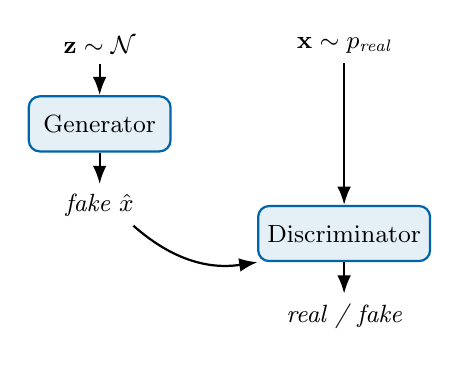
\begin{tikzpicture}[node distance=4mm,
            box/.style={draw=zhawaccent,thick,rounded corners,
                        minimum width=18mm,minimum height=7mm,
                        fill=zhawaccent!10,font=\small},
            data/.style={font=\small\itshape},
            arrow/.style={-Latex,thick}]
        \node[data] (z) {$\mathbf{z}\sim\mathcal{N}$};
        \node[box,below=of z] (G) {Generator};
        \node[data,below=of G] (fake) {fake $\hat{x}$};
        \node[data,right=18mm of z] (xreal)
            {$\mathbf{x}\sim p_{\text{real}}$};
        \node[box,below=18mm of xreal] (D) {Discriminator};
        \node[data,below=of D] (out) {real / fake};
        \draw[arrow] (z) -- (G);
        \draw[arrow] (G) -- (fake);
        \draw[arrow] (fake) to[bend right=25] (D);
        \draw[arrow] (xreal) -- (D);
        \draw[arrow] (D) -- (out);
        \end{tikzpicture}
        \end{center}
    \end{column}
    \end{columns}
\end{frame}

%----------------------------------------
\begin{frame}{How a classical generator produces correlated samples}
    Latent $\mathbf{z}\sim\mathcal{N}(0,I_{d_z})$ has independent
    components. The generator stacks affine maps and
    non-linearities:
    \[
    G(\mathbf{z}) = \tanh\bigl(W_3\,\sigma(W_2\,
    \sigma(W_1\mathbf{z}+\mathbf{b}_1)+\mathbf{b}_2)
    +\mathbf{b}_3\bigr), \quad \sigma = \text{LeakyReLU}
    \]
    \medskip

    All output correlations come from \emph{deterministic
    mixing of independent noise} via the learned weights:
    \[
    \mathrm{Cov}(y_i, y_j) \approx (W W^\top)_{ij},
    \quad W = W_3 W_2 W_1
    \]
    \medskip

    \begin{block}{Mechanism in one phrase}
        Output dependence is built entirely from
        \emph{deterministic mixing of independent noise}.
        Capacity to model complex joint structure scales with
        parameter count.
    \end{block}
\end{frame}

% !TEX root = ../main.tex

\section{The Quantum Generator}
\label{sec:quantum}
\frame[plain]{\sectionpage}

%----------------------------------------
\begin{frame}{From noise to market scenario: hybrid pipeline}
    \begin{center}
    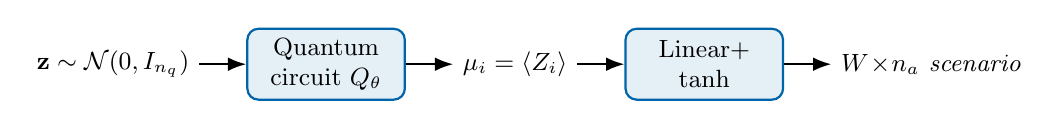
\begin{tikzpicture}[node distance=6mm,
        box/.style={draw=zhawaccent,thick,rounded corners,
                    minimum width=20mm,minimum height=9mm,
                    fill=zhawaccent!10,align=center,font=\small},
        data/.style={font=\small\itshape},
        arrow/.style={-Latex,thick}]
    \node[data] (z) {$\mathbf{z}\sim\mathcal{N}(0,I_{n_q})$};
    \node[box,right=of z] (Q) {Quantum\\circuit $Q_\theta$};
    \node[data,right=of Q] (mu) {$\mu_i = \langle Z_i\rangle$};
    \node[box,right=of mu] (h) {Linear+\\$\tanh$};
    \node[data,right=of h] (out)
        {$W\!\times\!n_a$ scenario};
    \draw[arrow] (z) -- (Q);
    \draw[arrow] (Q) -- (mu);
    \draw[arrow] (mu) -- (h);
    \draw[arrow] (h) -- (out);
    \end{tikzpicture}
    \end{center}
    \medskip

    \textbf{Two-stage architecture}
    \begin{itemize}
        \item \textbf{Quantum part} $Q_\theta:
        \mathbb{R}^{n_q}\to[-1,1]^{n_q}$ produces $n_q$
        expectation values via an entangled circuit
        \item \textbf{Classical head} upsamples to full output
        dimension via a single \texttt{Linear}~+~$\tanh$
    \end{itemize}
    \medskip

    \emph{Discriminator unchanged from the classical baseline.
    Only the generator differs --- a controlled comparison.}
\end{frame}

%----------------------------------------
\begin{frame}{The variational quantum circuit}
    \begin{columns}[T]
    \begin{column}{.55\textwidth}
        Operations on $\mathcal{H} = \mathbb{C}^{2^{n_q}}$:
        \medskip

        \begin{enumerate}
            \item \textbf{Initial state} $|\mathbf{0}\rangle$
            \item \textbf{AngleEmbedding}: apply $RY(z_i)$ on
            each qubit (encodes input as rotations)
            \item \textbf{Variational layer (×$L$)}:
            trainable $RY(\theta_{\ell,i})$ on each qubit, then
            a ring of CNOTs
            \item \textbf{Measure} $\mu_i = \langle Z_i\rangle
            \in [-1,1]$ on each qubit
        \end{enumerate}
        \medskip

        Total trainable angles: $n_q \times L$.\\
        For $n_q=8, L=3$: \textbf{24 quantum parameters} on a
        256-dim complex state space.
    \end{column}
    \hfill
    \begin{column}{.43\textwidth}
        \begin{block}{Why this design?}
            \begin{itemize}
                \item Hardware-efficient: nearest-neighbour
                CNOTs only
                \item $RY$-only rotations mitigate barren
                plateaus relative to richer
                ansätze~\cite{McClean2018BarrenPlateaus}
                \item Local Pauli-Z measurements bound
                gradient variance~\cite{Cerezo2021LocalCost}
                \item $L=3$: enough depth for entanglement to
                spread; deeper risks barren plateaus
            \end{itemize}
        \end{block}
    \end{column}
    \end{columns}
\end{frame}

% !TEX root = ../main.tex

\section{Entanglement and Joint Distributions}
\label{sec:entanglement}
\frame[plain]{\sectionpage}

%----------------------------------------
\begin{frame}{What entanglement provides}
    \textbf{Without entanglement} (single-qubit gates only): the
    state stays a product
    $|\psi\rangle = |\psi_1\rangle\otimes\cdots\otimes
    |\psi_{n_q}\rangle$ and measurements are
    \emph{statistically independent}:
    \[
    P(\mu_1,\ldots,\mu_{n_q}) = \prod_i P(\mu_i)
    \]
    \medskip

    \textbf{With CNOTs}: state is no longer separable. Joint
    structure that no product distribution can reproduce.
    \medskip

    \begin{block}{Bell state example}
        Two qubits, Hadamard on qubit 1, then CNOT:
        \[
        |0\rangle\otimes|0\rangle \;\longrightarrow\;
        \tfrac{1}{\sqrt 2}(|00\rangle+|11\rangle)
        \]
        Marginals: $\langle Z_1\rangle = \langle Z_2\rangle = 0$
        (uniform random).
        Joint: $\langle Z_1 Z_2\rangle = +1$ (perfectly
        correlated). No product of independent random variables
        can produce this.
    \end{block}
\end{frame}

%----------------------------------------
\begin{frame}{Two routes to correlated samples}
    \begin{columns}[T]
    \begin{column}{.48\textwidth}
        \textbf{Classical generator}\\
        Independent noise $\mathbf{z}$\\
        $\downarrow$ deterministic mixing\\
        $\downarrow$ via learned $W_1, W_2, W_3$\\
        $\downarrow$\\
        Correlated outputs
        \medskip

        All correlation must be encoded in the weight
        matrices.
    \end{column}
    \hfill
    \begin{column}{.48\textwidth}
        \textbf{Hybrid quantum generator}\\
        Independent noise $\mathbf{z}$\\
        $\downarrow$ entangled circuit\\
        $\downarrow$ produces correlated $(\mu_1,\ldots,\mu_{n_q})$\\
        $\downarrow$\\
        Classical head upsamples
        \medskip

        Quantum part introduces dependence between features
        \emph{before} the head sees them.
    \end{column}
    \end{columns}
    \medskip

    \begin{center}
    \emph{Hypothesis: this should make the hybrid generator
    \textbf{more parameter-efficient} for joint distributions ---
    a claim our project tests empirically.}
    \end{center}
\end{frame}

%----------------------------------------
\begin{frame}{What this is, and is not, a claim of}
    \begin{columns}[T]
    \begin{column}{.48\textwidth}
        \textbf{We claim, theoretically:}
        \begin{itemize}
            \item Entanglement provides an architectural
            \emph{pathway} for joint structure that
            classical mixing does not have natively
            \item The set of joint distributions reachable
            by depth-$L$ quantum circuits differs from the
            set reachable by classical NNs of comparable
            parameter count
        \end{itemize}
    \end{column}
    \hfill
    \begin{column}{.48\textwidth}
        \textbf{We do not claim:}
        \begin{itemize}
            \item That classical NNs cannot represent
            these distributions (they can, given enough
            capacity)
            \item That parameter-efficiency manifests in
            every regime
            \item That entanglement is the \emph{only}
            possible explanation for any observed effect
        \end{itemize}
    \end{column}
    \end{columns}
    \medskip

    \begin{center}
    \emph{The honest framing: a hypothesis we test, not a theorem
    we prove.}
    \end{center}
\end{frame}

% !TEX root = ../main.tex

\section{Evaluation Methodology}
\label{sec:evaluation}
\frame[plain]{\sectionpage}

%----------------------------------------
\begin{frame}{What we measure}
    Generator output: a $W \times n_a$ array of log-returns.
    Three families of metrics:
    \medskip

    \textbf{1.\ Marginal statistics} (per asset)
    \begin{itemize}
        \item Mean, std, skewness, excess kurtosis
        \item Two-sample Kolmogorov-Smirnov distance
    \end{itemize}
    \medskip

    \textbf{2.\ Joint dependence} ($n_a \geq 2$)
    \begin{itemize}
        \item Pearson correlation matrix
        \item Frobenius distance on correlation matrices
    \end{itemize}
    \medskip

    \textbf{3.\ Computational cost}
    \begin{itemize}
        \item Trainable parameter count (quantum vs classical
        breakdown)
        \item Wall-clock training time
    \end{itemize}
\end{frame}

%----------------------------------------
\begin{frame}{Experimental design}
    \begin{columns}[T]
    \begin{column}{.48\textwidth}
        \textbf{Data}
        \begin{itemize}
            \item Daily closes 2005--2024 (Yahoo Finance)
            \item Log-returns, scaled to $\sim[-1,1]$ per asset
            \item Windows of 20 trading days (rolling, stride 1)
            \item Chronological 80/20 train/test split
        \end{itemize}
        \medskip

        \textbf{Configurations}
        \begin{itemize}
            \item Multivariate, 5 assets:\\
            \smi, \dax, EuroStoxx, FTSE, \sap
            \item Vanilla GAN training
            \item Quantum: $n_q \in \{6,8,10,12\}$,
            $L=3$ layers
        \end{itemize}
    \end{column}
    \hfill
    \begin{column}{.48\textwidth}
        \textbf{Controlled comparison}\\
        Identical across all runs:
        \begin{itemize}
            \item Discriminator architecture
            \item Loss function, optimiser, hyperparameters
            \item Seed, evaluation pipeline, data
        \end{itemize}
        \medskip

        Only the generator differs; any observed difference is
        attributable to the generator architecture --- and within
        the quantum case, to the entanglement that creates joint
        feature structure before the classical head.
    \end{column}
    \end{columns}
\end{frame}


%----------------------------------------
%   RESULTS
%----------------------------------------
% !TEX root = ../main.tex

\section{Results}
\label{sec:results}
\frame[plain]{\sectionpage}

%----------------------------------------
\begin{frame}{Headline comparison: classical vs hybrid quantum}
    Multivariate vanilla GAN, 5 assets
    (\smi, \dax, EuroStoxx, FTSE, \sap), best quantum at $n_q=10$:
    \medskip

    \begin{center}
    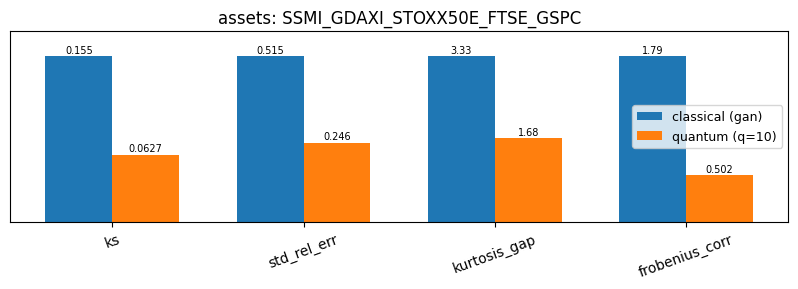
\includegraphics[width=0.85\textwidth]{comparison_classical_vs_quantum}
    \end{center}
    \medskip

    \textbf{Quantum wins on all four metrics}, with parameter
    count comparable: 4644 (classical) vs 1130 ($n_q=10$).
    Largest effect on cross-asset correlation
    (Frobenius $1.79 \to 0.50$, $\sim\!3.6\!\times$ improvement).
\end{frame}

% !TEX root = ../main.tex

%----------------------------------------
\begin{frame}{Marginal distributions: shape and tails}
    \begin{columns}[T]
    \begin{column}{.45\textwidth}
        Per-asset histograms of log-returns
        (real vs.\ classical vs.\ $q=6, 10$):
        \medskip

        \textbf{Quantum tracks the real bulk closely}; peaks
        slightly too tall (under-dispersed).
        \medskip

        \textbf{Classical} learns a much wider distribution
        and overshoots the tails --- explains the
        $0.515$ standard error vs.\ $0.246$ for quantum.
        \medskip

        \emph{Same qualitative pattern across all 5 assets.}
    \end{column}
    \hfill
    \begin{column}{.50\textwidth}
        \begin{center}
        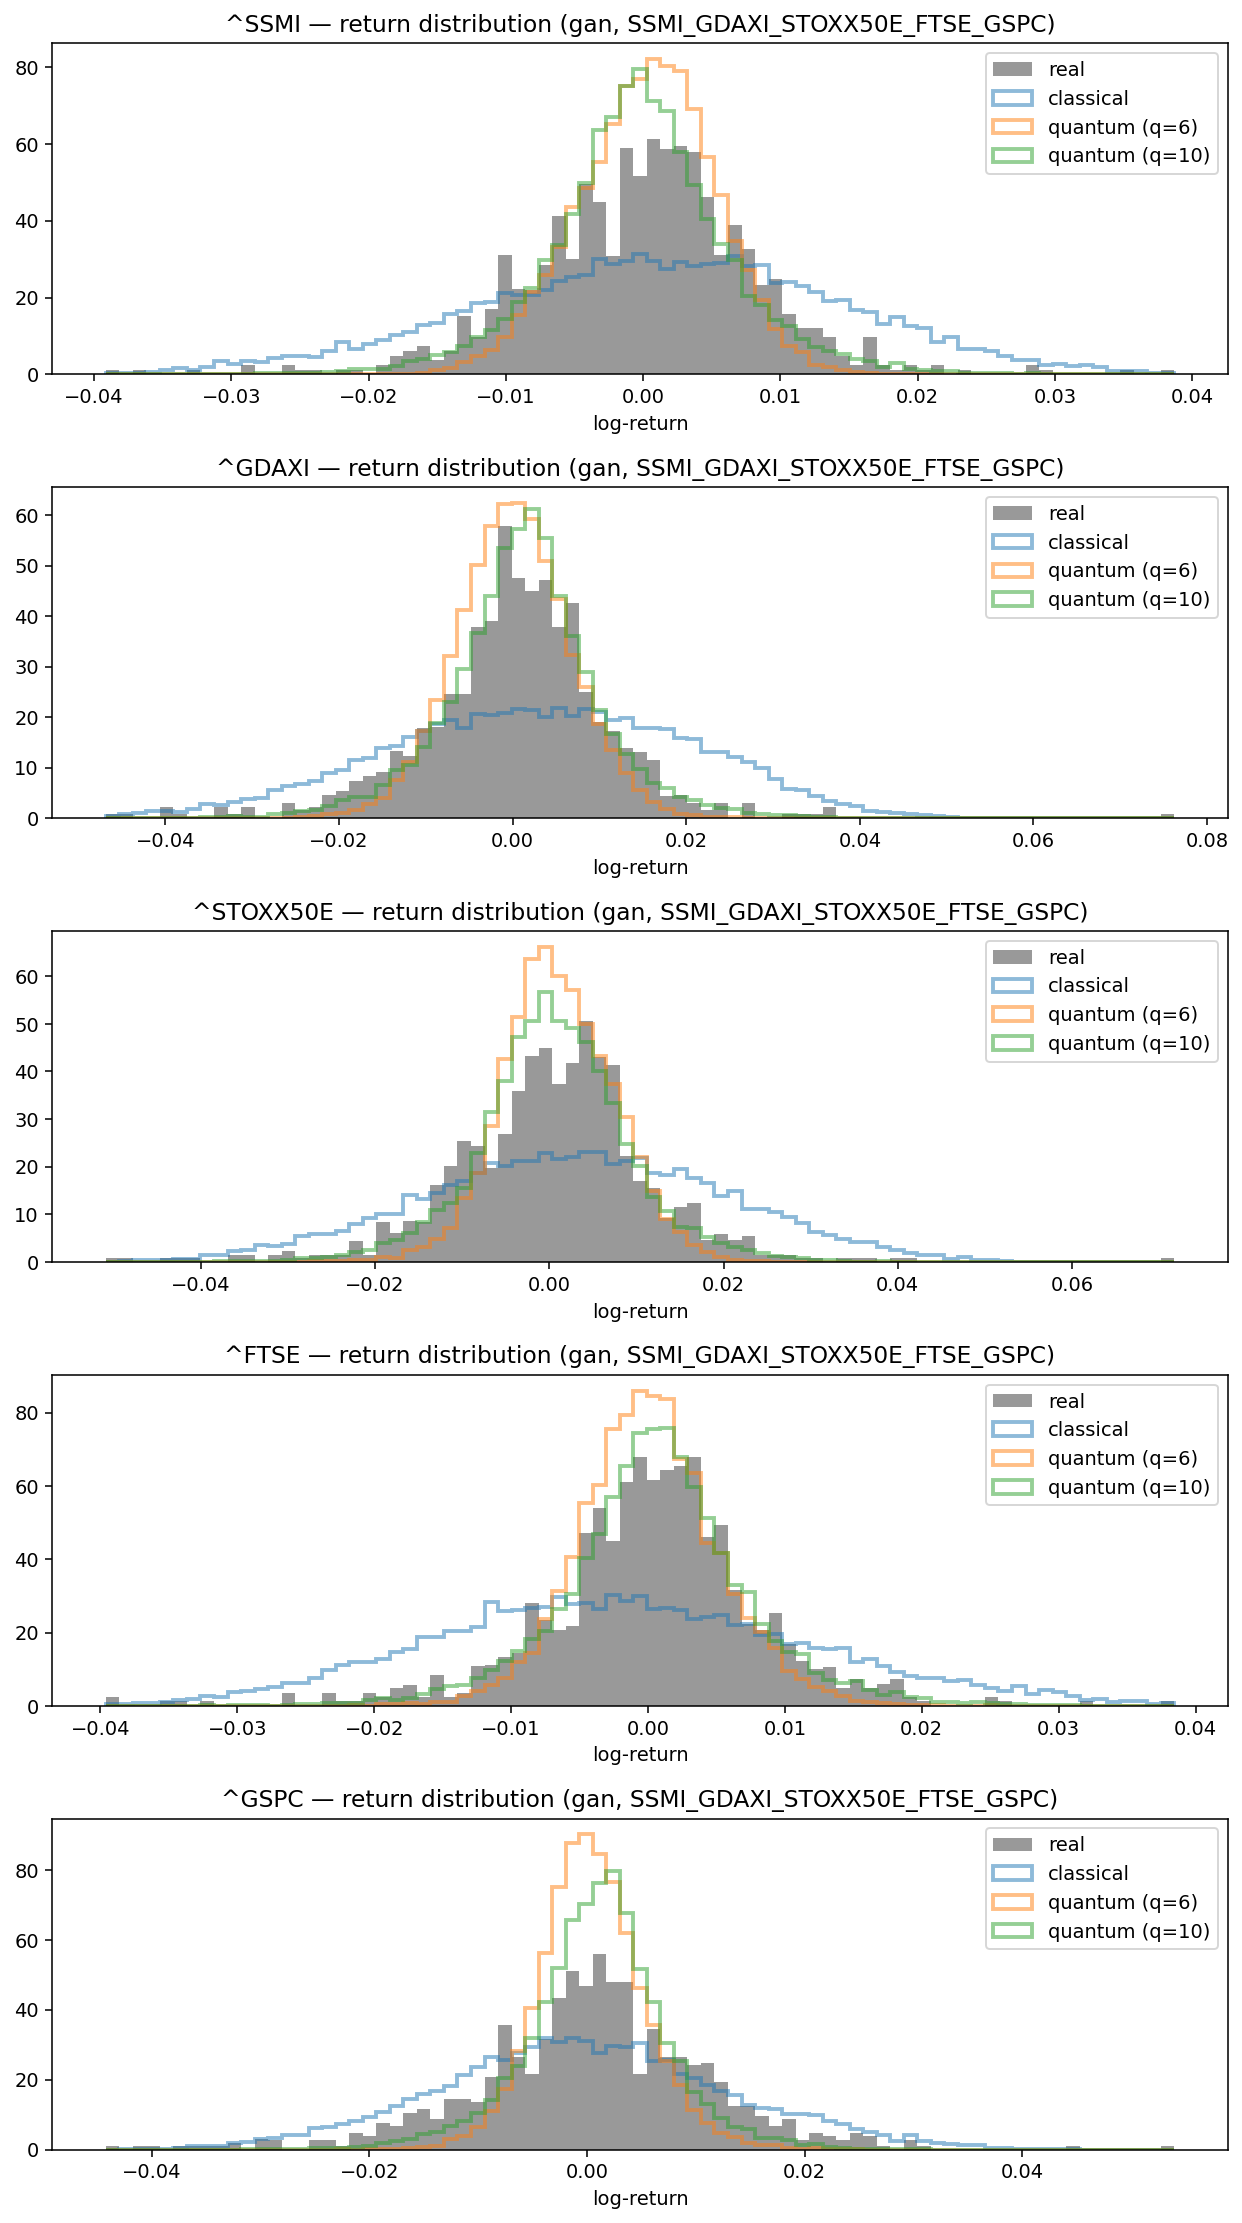
\includegraphics[height=0.85\textheight]{distributions_classical_vs_quantum}
        \end{center}
    \end{column}
    \end{columns}
\end{frame}

% !TEX root = ../main.tex

%----------------------------------------
\begin{frame}{Cross-asset correlation}
    \begin{center}
    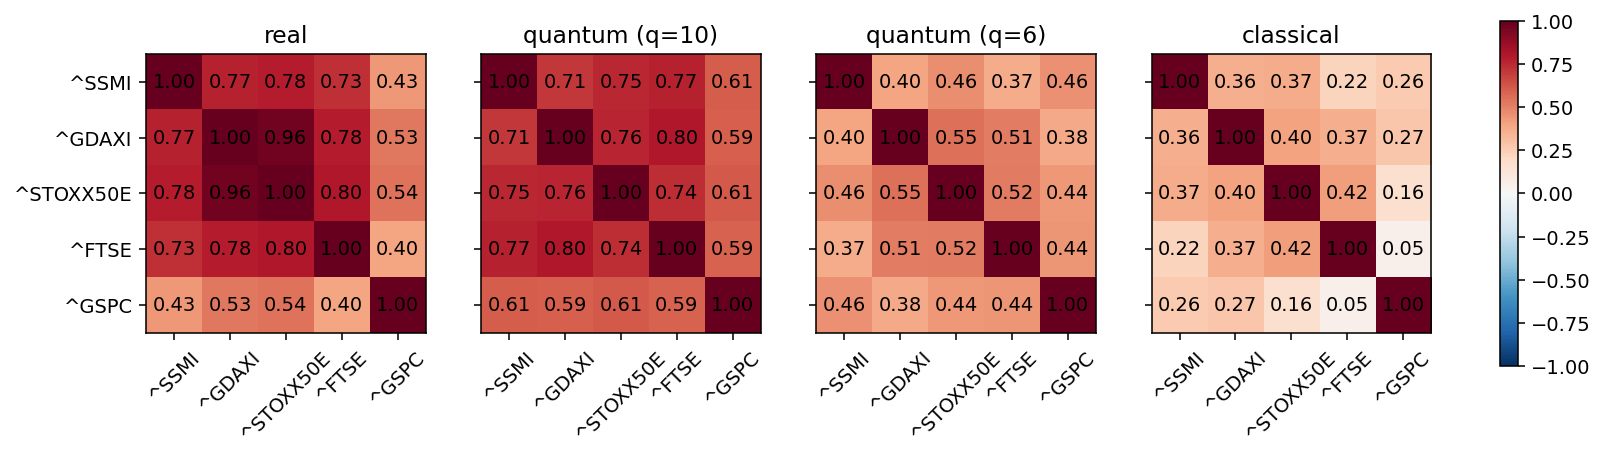
\includegraphics[width=0.95\textwidth]{correlation_classical_vs_quantum}
    \end{center}
    \medskip

    \begin{columns}[T]
    \begin{column}{.50\textwidth}
        \textbf{Real correlations} (left): strong European
        block %($\rho \!\sim\! 0.77\text{--}0.96$), 
        weaker US--Europe link %($\rho \!\sim\! 0.4\text{--}0.5$).
    \end{column}
    \hfill
    \begin{column}{.45\textwidth}
        \textbf{Quantum $n_q\!=\!10$} approximates both blocks.
        \textbf{Classical} collapses the European block;
        %($\rho \!\sim\! 0.2\text{--}0.4$) --- 
        the joint structure is largely lost.
    \end{column}
    \end{columns}
\end{frame}

% !TEX root = ../main.tex

\section{Qubit Scaling}
\label{sec:scaling}
\frame[plain]{\sectionpage}

%----------------------------------------
\begin{frame}{Qubit-count scaling: an empirical barren-plateau signature}
    Multivariate vanilla GAN, 5 assets, $n_q \in \{6,8,10,12\}$:
    \medskip

    \begin{center}
    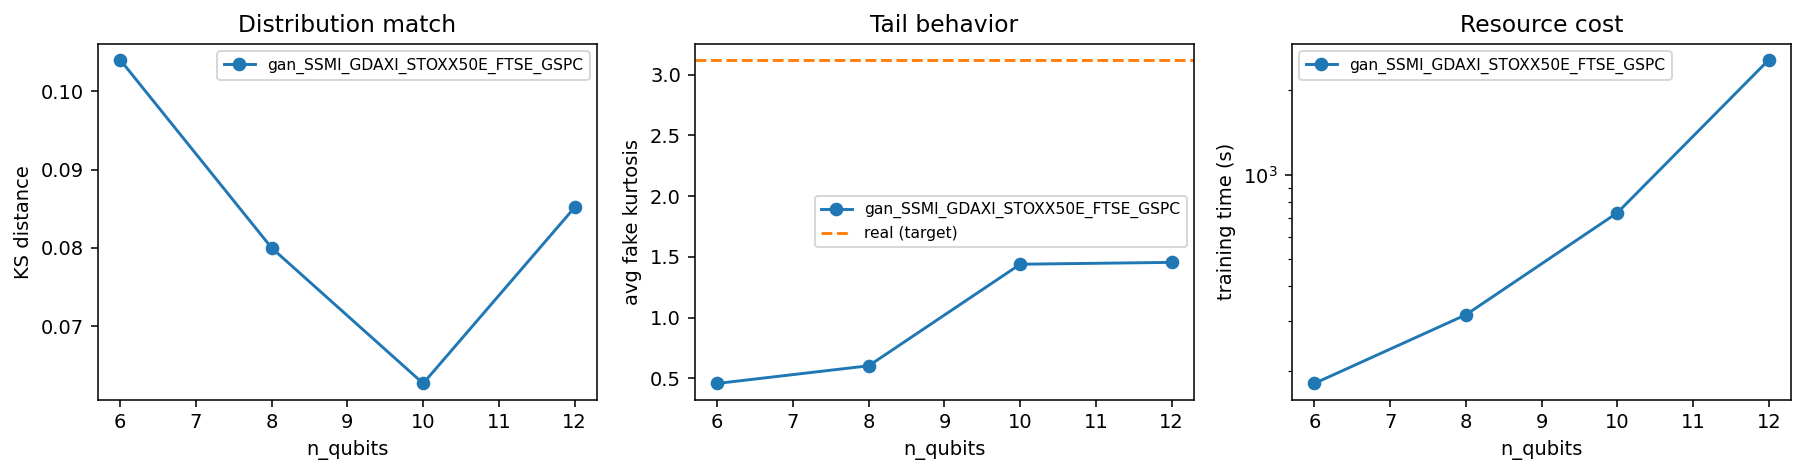
\includegraphics[width=0.95\textwidth]{qubit_scaling}
    \end{center}
    \medskip

    \textbf{Three observations:}
    \begin{itemize}
        \item KS \emph{improves} from $n_q\!=\!6$ to $n_q\!=\!10$,
        then \emph{degrades} at $n_q\!=\!12$
        % ($0.063 \!\to\! 0.085$)
        \item Tail kurtosis improves with $n_q$ but plateaus
        below the real target %($\sim\!1.5$ vs.\ $\sim\!3.1$)
        \item Training cost grows at increasing rate:
        $\sim\!14\!\times$ slower at $n_q\!=\!12$ than $n_q\!=\!6$
    \end{itemize}
    \medskip

    The $n_q\!=\!12$ degradation is consistent with the
    \emph{barren plateau} phenomenon~\cite{McClean2018BarrenPlateaus}.
\end{frame}

% !TEX root = ../main.tex

\section{Discussion}
\label{sec:discussion}
\frame[plain]{\sectionpage}

%----------------------------------------
\begin{frame}{What we found, what we did not}
    \begin{columns}[T]
    \begin{column}{.48\textwidth}
        \textbf{What we found}
        \begin{itemize}
            \item Hybrid quantum GAN outperforms classical
            on all four metrics (KS, std, kurtosis,
            cross-correlation)
            \item Largest effect on \emph{joint dependence}
            %($\sim\!3.6\!\times$ lower Frobenius error)
            \item Quality improves with $n_q$ up to a clear
            optimum %($n_q\!=\!10$ in our setup)
        \end{itemize}
    \end{column}
    \hfill
    \begin{column}{.48\textwidth}
        \textbf{What we did not find}
        \begin{itemize}
            \item No monotone improvement past $n_q\!=\!10$:
            $n_q\!=\!12$ degrades, consistent with barren
            plateaus
            \item Tail behavior not fully recovered:
            fake kurtosis $\sim\!1.5$ vs.\ real $\sim\!3.1$%,
            % limited by the $\tanh$ output bottleneck
            \item Quantum simulation cost
            ($\sim\!10\text{--}100\!\times$ slower than
            classical) makes routine deployment impractical
        \end{itemize}
    \end{column}
    \end{columns}
    \medskip

    % \textbf{Honest framing.} The observed advantage is consistent
    % with the entanglement-as-joint-structure hypothesis, but
    % not isolated from it: a fully matched-parameter classical
    % baseline with no entanglement remains a natural follow-up.
\end{frame}

%----------------------------------------
\begin{frame}{Take-aways}
    \begin{itemize}
        \item Replacing the GAN \emph{generator} with a small
        variational quantum circuit produces measurably
        \emph{better} cross-asset distributional structure on a
        controlled 5-asset benchmark.

        \item The dimensionality argument has empirical support:
        the quantum advantage is largest where joint structure
        matters most (correlation, not marginal tails).

        \item Naive intuition about scaling fails:
        more qubits do not necessarily improve performance --
        an optimization barrier (barren plateaus) bounds
        the usable regime.

        % \item Practical deployment requires the tools from
        % Lecture~6: \emph{local costs, problem-informed ans\"atze,
        % warm initialisation} --- precisely what the next
        % iteration of this project would need.
    \end{itemize}
    \medskip

    \begin{center}
    \emph{Code, data, and figures:}\\
    \url{github.com/wuns/qGAN-market-generator}{github.com/wuns/qGAN-market-generator}
    \end{center}
\end{frame}


%----------------------------------------
%   BIBLIOGRAPHY
%----------------------------------------
\begin{frame}[allowframebreaks]{References}
\printbibliography
\end{frame}

\end{document}
